\documentclass[11pt,a4paper]{article}

\usepackage[utf8]{inputenc}
\usepackage[T1]{fontenc}
\usepackage{lmodern}
\usepackage[english]{babel}
\usepackage{geometry}
\usepackage{graphicx}
\usepackage{float}
\usepackage{hyperref}

\geometry{margin=2.5cm}

\begin{document}

\begin{titlepage}
    \centering
    \vspace*{1.5cm}

    {\Large \textbf{Web Application Project}\par}
    \vspace{0.3cm}
    {\Large \textbf{Project Topic: Lie Detector Arena}\par}
    \vspace{0.6cm}
    {\large \textbf{Progress Report -- Iteration 3}\par}

     \vspace{2.8cm}

    {\large \textbf{Project Team}\par}
     \vspace{0.5cm}

    {\Large \textbf{Mohamed Radhi}\par
     \vspace{0.15cm}
     \textbf{Amina Kamal}\par
     \vspace{0.15cm}
     \textbf{Houssem Trabelsi}\par
     \vspace{0.15cm}
     \textbf{Rayane Kohil}\par}

     \vspace{2.8cm}

    {\large \textbf{April 28, 2026}\par}

    \vfill

    {\large \textbf{ENSEEIHT -- Web Application Project}\par}
\end{titlepage}

\section{Overview}

This iteration focused on finishing remaining backend features, stabilizing game-cycle logic, and integrating final-game awards and lifetime profile updates. The goal was to clear schema migration issues, ensure tests pass, and expose endpoints the frontend needs to render final results and awards.

\section{Implemented Components and Recent Changes}

\subsection{Repository Interfaces}

The repository interfaces support persistence layer queries and were extended where needed:

\begin{itemize}
    \item \texttt{ChatMessageRepository}: manages chat messages by round
    \item \texttt{GameRepository}: retrieves games by room
    \item \texttt{InvitationRepository}: finds invitations by room or receiver
    \item \texttt{PlayerProfileRepository}: retrieves profiles by player
    \item \texttt{ScoreEntryRepository}: finds scores by game or player
\end{itemize}

\subsection{Service Classes}

Core service classes handle business logic for the game domain; notable additions and changes in this iteration include:

\begin{itemize}
    \item \texttt{GameAwardsService}: computes per-game awards and applies lifetime profile updates (one-time) when a game completes
    \item Cycle-aware enhancements to \texttt{RoundService} and \texttt{GameService} to support multi-cycle speaker rotation and auto-progression
    \item Defensive updates across services to handle empty collections and reduce fragility when the HSQL file is locked by OneDrive
\end{itemize}

\subsection{REST Controllers}

REST controllers expose service functionality. This iteration added or updated endpoints used by the frontend (examples):

\begin{itemize}
    \item \texttt{GameController}: now exposes \texttt{/api/games}, \texttt{/api/games/{id}/speaker-progress}, and \texttt{/api/games/{id}/final-summary}
    \item \texttt{GameRoomController}: \texttt{/rooms/{id}/players} returns room player summaries to avoid fragile nested graph serialization
\end{itemize}

Each controller follows REST conventions: \texttt{POST} for creation, \texttt{GET} for retrieval, with support for filtering by related entities.

\subsection{Backend Tests and Status}

The test suite covers unit and slice tests; important outcomes from this iteration:

\begin{itemize}
    \item Unit tests: \texttt{UserServiceTest}, \texttt{GameRoomServiceTest}, and others were maintained and extended
    \item Controller slice tests: \texttt{BackendControllersTest} uses mocked beans via a test configuration; recent mocks were added for new dependencies such as \texttt{GameAwardsService}
\end{itemize}

All tests use Mockito for service mocking and Spring MockMvc for HTTP testing. After addressing an HSQLDB migration issue (see below), the backend test run completed successfully (local run: 18 tests, BUILD SUCCESS).

\section{Domain Model}

The domain model supporting this iteration includes the main entities: users, players, player profiles, game rooms, games, rounds, statements, votes, chat messages, invitations, and score entries.

\begin{figure}[H]
    \centering
    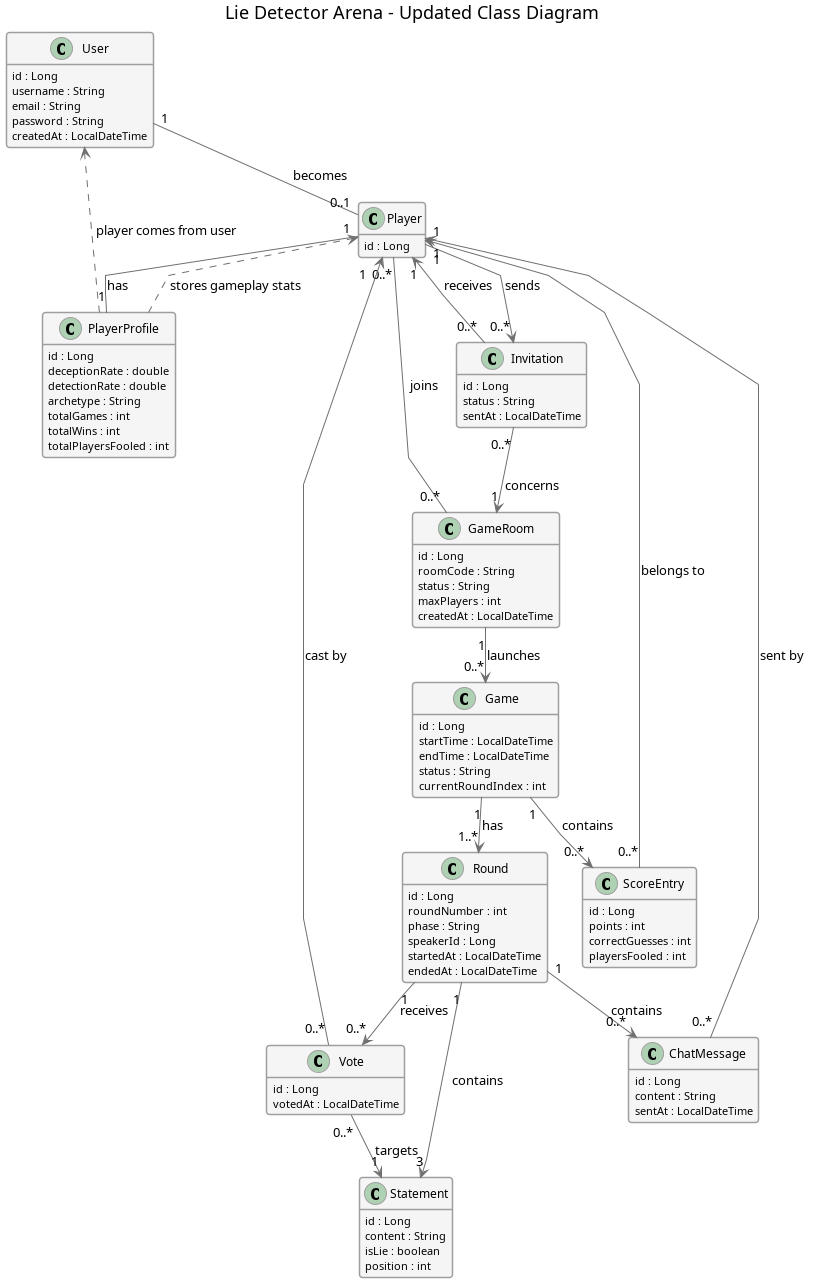
\includegraphics[width=\textwidth]{class_diagram_iteration2.png}
    \caption{Class diagram of the Lie Detector Arena domain model}
    \label{fig:class-diagram}
\end{figure}

\section{Result}

The backend is now feature-complete for the current game model and includes the following key updates:

\begin{itemize}
    \item All main REST controllers and services are implemented and wired
    \item \texttt{GameAwardsService} computes final-game awards and applies profile lifetime stats exactly once per completed game
    \item Cycle configuration (default 2, max 10) added to the game creation flow (frontend and backend)
    \item Migration fix applied so HSQLDB schema updates succeed for newly added non-null fields
    \item Backend tests run clean locally after fixes
\end{itemize}

The REST API is ready for the frontend to consume final-summary data and awards.

\section{Notable Changes and Fixes}

\begin{itemize}
    \item \textbf{Cycle and UX:} Results page auto-cycle countdown implemented (UX preference: 3s with visible countdown; earlier local test used 5s)
    \item \textbf{Cycle configuration:} Game creation UI accepts a \texttt{cycles} parameter (default 2, max 10) and backend persists \texttt{targetCycles}
    \item \textbf{Final awards:} \texttt{GameAwardsService} computes awards, applies tie-break logic (better liar wins; equal liar quality => tie), and updates lifetime metrics (`gamesPlayed`, `gamesWon`, `gamesLost`) in \texttt{PlayerProfile}
    \item \textbf{Migration fix:} HSQLDB required an explicit default for new non-null columns. The following change was applied to \texttt{PlayerProfile} to avoid alter-table errors:
    \begin{verbatim}
    @Column(nullable = false, columnDefinition = "integer default 0")
    private int totalLosses;
    \end{verbatim}
    This prevents the "default expression needed" error during schema update.
    \item \textbf{Tests:} \texttt{BackendControllersTest} test config was adjusted to mock \texttt{GameAwardsService}; backend tests passed after fixes.
\end{itemize}

\section{Next Steps}

\begin{itemize}
    \item Verify the \texttt{final-summary} endpoint end-to-end with a completed game and confirm awards rendering in the Results UI (frontend)
    \item Add integration tests that exercise full game completion and ensure lifetime profile updates are idempotent
    \item Polish final awards UX (countdown timing, animation, tie-break presentation) and merge frontend changes
    \item Add DTO-level validation and consider authentication/authorization for production deployment
\end{itemize}

\end{document}